\documentclass[conference]{IEEEtran}
\IEEEoverridecommandlockouts
\usepackage{cite}
\usepackage{amsmath,amssymb,amsfonts}
\usepackage{algorithmic}
\usepackage{graphicx}
\usepackage{textcomp}
\usepackage{xcolor}
\usepackage{booktabs}
\usepackage{multirow}
\def\BibTeX{{\rm B\kern-.05em{\sc i\kern-.025em b}\kern-.08em
    T\kern-.1667em\lower.7ex\hbox{E}\kern-.125emX}}
\begin{document}

\title{Performance Evaluation of Post-Quantum Digital Signatures for C-V2X Sidelink Communications}

%\title{Comparative Performance Evaluation of Classical and Post-Quantum Digital Signatures on C-V2X Sidelink Communications}

% \author{
%  \IEEEauthorblockN{Akid Abrar\IEEEauthorrefmark{1}, Sagar Dasgupta\IEEEauthorrefmark{1},
%   Abdullah Al Mamun\IEEEauthorrefmark{2}, Mizanur Rahman\IEEEauthorrefmark{1},
%   Mashrur Chowdhury\IEEEauthorrefmark{2}, Ahmad Alsharif\IEEEauthorrefmark{7}}
%   \IEEEauthorblockA{\IEEEauthorrefmark{1}Department of Civil, Construction \& Environmental Engineering, The University of Alabama, Tuscaloosa, AL, USA}
%   \IEEEauthorblockA{\IEEEauthorrefmark{2}Glenn Department of Civil Engineering,
%   Clemson University, Clemson, SC, USA}
%   \IEEEauthorblockA{\IEEEauthorrefmark{7}Department of Computer Science, The University of Alabama, Tuscaloosa, AL, USA}
% }


\maketitle

\begin{abstract}
The recent and anticipated advent of quantum computing poses a threat to the Elliptic Curve Cryptography (ECC)-based classical digital signatures that secure cellular Vehicle-to-Everything (C-V2X) sidelink communication following current IEEE 1609.2 vehicular security standards. Post-quantum cryptographic (PQC) algorithms offer resistance to known quantum attacks but introduce significantly larger signature and key sizes compared to classical digital signature algorithms. Existing studies lack a comparative performance evaluation of PQC and classical digital signatures that accounts for realistic vehicular traffic conditions, C-V2X sidelink radio resource constraints, and safety application requirements. This paper develops a comparative performance evaluation strategy and conducts a quantitative assessment between the classical Elliptic Curve Digital Signature Algorithm (ECDSA) and Falcon-512 for C-V2X Mode 4 sidelink communications. Falcon-512 is a lattice-based PQC digital signature scheme selected by the National Institute of Standards and Technology (NIST) for standardization. We have quantified the sidelink communication impact of Falcon-512's larger signature and public key sizes through two key performance indicators, packet delivery ratio (PDR) and end-to-end latency, under moderate urban roadway vehicular traffic density. The analysis indicates that Falcon-512 and ECDSA exhibit nearly identical average latencies of around 52 ms. However, the 470\% increase in packet size for Falcon-512 compared to ECDSA lowers the average PDR from 95\% to 71\%. The PDR and end-to-end latency analysis demonstrate that spectrum efficiency, rather than computational cost, is the primary bottleneck for PQC adoption in bandwidth-constrained C-V2X networks.
\end{abstract}

\begin{IEEEkeywords}
Post-quantum cryptography, C-V2X, Mode 4, Falcon-512, performance evaluation
\end{IEEEkeywords}

\section{Background and Motivation}

Cellular-Vehicle-to-Everything (C-V2X) communication enables vehicles to exchange safety-critical messages, such as Basic Safety Messages (BSMs) via the PC5 Mode 4 sidelink interface without cellular infrastructure~\cite{3gpp_36213}. The IEEE~1609.2 standard specifies the Elliptic Curve Digital Signature Algorithm (ECDSA), utilizing the National Institute of Standards and Technology (NIST) P-256 curve for message authentication. ECDSA generates a 64-byte signature and a 65-byte public key~\cite{ieee_16092}. However, Shor's algorithm can break ECDSA using a Cryptographically Relevant Quantum Computer (CRQC)~\cite{shor1994algorithms}, necessitating migration to post-quantum cryptographic (PQC) alternatives~\cite{mamun_pqc}.

NIST published Module-Lattice-Based Digital Signature Algorithm (ML-DSA), also known as Dilithium, as Federal Information Processing Standards (FIPS) 204 in August 2024 \cite{fips204}. The Fast Fourier Transform (FFT) over N-th degree Truncated Polynomial Ring Units (NTRU)-Lattice-Based Digital Signature Algorithm (FN-DSA), also known as Falcon, has been selected by NIST for standardization as FIPS 206, with finalization pending as of this writing \cite{nist_pqc_2024}. Falcon-512 is the most compact among the NIST-standardized post-quantum signature candidates. Still, its signature and public key size inflation compared to the ECDSA creates significant strain on the sidelink transport block capacity within the system configuration specified by the Society of Automotive Engineers (SAE) J3161 standard \cite{sae_j3161}. Within this configuration, a single Secure Protocol Data Unit (SPDU) defined in IEEE 1609.2 containing a Falcon-512 signature requires multiple subchannels per transmission and substantially increases total spectrum usage in dense roadway vehicular traffic.

C-V2X PC5 Mode 4 is a decentralized semi-persistent sidelink communication mode in which vehicles autonomously select radio resources from a shared spectrum pool without centralized cellular infrastructure. Unlike cellular-infrastructure-assisted communication systems (PC5 Mode 3), where scheduling and resource allocation can be centrally coordinated, each vehicle independently performs resource selection based on locally sensed channel occupancy~\cite{hajisami2022tutorial}. The communication overhead associated with PQC authentication is critically important in this context because the increased in packet size directly affects not only the transmitting node (e.g., vehicle) but also the overall channel resource availability observed by neighboring nodes (e.g., vehicles). This trade-off between cryptographic payload size and shared radio resource utilization creates a sophisticated systems-level challenge for PQC migration in vehicular networks.

Safety-critical vehicular applications, such as intersection collision avoidance, emergency electronic brake light warnings, and platooning, require frequent low-latency message exchange with high delivery reliability. These applications typically operate under strict communication constraints because messages must be repeatedly broadcast to all nearby nodes at high transmission frequencies. Therefore, an increase in message size can significantly affect communication channel congestion, packet collision probability, and communication scalability when traffic density becomes sufficiently high~\cite{hajisami2022tutorial}.

Among the currently standardized PQ digital signature candidates, Falcon-512 provides the smallest signature sizes and therefore represents a lower-bound estimate of the communication overhead expected from PQC migration in vehicular networks~\cite{mamun_pqc}. Alternative NIST-standardized schemes, such as Dilithium and SPHINCS+, produce substantially larger signatures~\cite{mamun_pqc} and would likely impose even greater performance degradation under sidelink resource constraints. Consequently, evaluating Falcon-512 provides an important baseline for understanding the feasibility limits of PQC authentication in bandwidth-constrained C-V2X communication systems.

% Add Twardokus's 1st paper
Prior works on PQC for vehicular networks have mainly focused on embedded computational overhead, protocol integration, and emerging cross-layer authentication designs. Sinell et al.~\cite{sinell2025evaluation} evaluated Falcon on automotive-grade Infineon AURIX TC399 multicore hardware and found that signature verification executes quickly, which is suitable for real-time use, whereas both key pair and signature generation exhibit long and highly variable execution times, rendering them unsuitable for typical automotive real-time constraints. Barreto et al.~\cite{barreto2018qscms} proposed qSCMS, a lattice-based post-quantum extension of the V2X Security Credential Management System (SCMS), but did not evaluate sidelink radio performance. Twardokus and Rahbari~\cite{twardokus2025chasm} proposed CHASM, a hybrid quantum-resistant C-V2X authentication protocol that combines certificate fragmentation and adaptive modulation to reduce the communication overhead of large PQC certificates. While their work validates a cross-layer mitigation strategy under varying communication densities, it does not model traffic operations through a microscopic mobility simulator or quantify how replacing ECDSA with Falcon-512 affects C-V2X performance in high-volume vehicular traffic scenarios in a roadway environment. This study addresses that gap by evaluating an urban intersection with moderate traffic density using an integrated co-simulation framework combining Objective Modular Network Testbed in C++ (OMNeT++) \cite{varga2008overview}, Vehicles in Network Simulation (Veins) \cite{sommer2019veins}, and Simulation of Urban Mobility (SUMO) \cite{behrisch2011sumo}. This framework evaluates ECDSA and Falcon-512 under controlled and identical conditions, including vehicular traffic load, channel model, Mode 4 autonomous resource selection, and certificate transmission pattern. By doing so, it isolates how Falcon-512’s larger SPDU size affects PDR and end-to-end latency under realistic C-V2X distributed sidelink resource allocation between vehicles and roadside units (RSUs) in an urban roadway intersection.

To address the lack of comparative performance evaluations of PQC and classical digital signatures under realistic roadway vehicular traffic flows, this paper develops and applies a comparative evaluation strategy for C-V2X Mode 4 sidelink communications. The strategy accounts for vehicular communication and security standards, C-V2X sidelink radio resource constraints, and safety-critical application-level requirements and is used to quantitatively compare classical ECDSA and Falcon-512 using SAE J3161-compliant simulation parameters to ensure alignment with current vehicular communication standards. The objective is to quantify the communication-level impact of PQC digital signatures under realistic sidelink resource constraints and determine whether the smallest among the currently standardized PQC digital signature alorithms can satisfy the reliability and latency requirements of safety-critical vehicular applications without requiring any substantial modifications to existing communication and security standards. We focus on assessing whether Falcon-512's large payloads can be accommodated within sidelink transport blocks without modifications to the message coding scheme (MCS) or subchannel limits and on quantifying the impact on PDR and end-to-end latency compared to the ECDSA. We have measured PDR as a function of distance using the 5GAA sliding-window evaluation approach \cite{5gaa_p190033}. This foundational evaluation demonstrates practical feasibility and guides the design of more comprehensive studies covering additional PQC candidates and roadway traffic scenarios.

\section{Method}
\label{sec: method}

To quantify the sidelink communication impact of post-quantum digital signatures, this study implements a five-stage evaluation strategy, outlined in Figure~\ref{fig:method}, comparing ECDSA P-256 and Falcon-512 under identical C-V2X Mode 4 conditions. First, a co-simulation environment is established by coupling an OMNeT++-based C-V2X Mode 4 simulator, OpenCV2X~\cite{opencv2x}, which is an extension of SimuLTE\cite{virdis2014simulte}, with the microscopic traffic simulator SUMO through Veins and its TraCI interface, enabling realistic co-simulation of vehicular communication and mobility. Second, two digital signature schemes are integrated into the communication stack under identical channel and mobility conditions: ECDSA P-256 as the classical baseline and Falcon-512 as the post-quantum baseline, so that any performance difference can be attributed solely to the change in cryptographic payload. Signatures are generated for every transmitted BSM. The full public key certificate is transmitted once every five BSMs, while the certificate digest is transmitted in the remaining four messages as per IEEE 1609.2 ~\cite{ieee_16092}. Third, the C-V2X Mode 4 sidelink channel and MAC-layer parameters are configured for line-of-sight propagation following SAE J3161. Fourth, the urban traffic scenario is instantiated in SUMO to reflect realistic traffic scenario, including vehicle density and speed distribution. Fifth, simulation outputs are post-processed to evaluate packet delivery ratio and end-to-end latency as performance indicators. This controlled comparison strategy allows the observed performance changes to be attributed primarily to the cryptographic payload expansion rather than to differences in mobility, propagation, or radio configuration.

The Falcon-512 signature scheme is constructed over NTRU lattices and leverages Fast Fourier Sampling \cite{fouque2017falcon}. It offers NIST security level 1, equivalent in strength to Advanced Encryption Standard (AES)-128, with the smallest combined signature and public key size among NIST-standardized PQC digital signature schemes. For example, compared with ML-DSA-44 (Dilithium-2), which has a 1,312-byte public key and a 2,420-byte signature, Falcon-512 has a smaller 897-byte public key and a 666-byte signature. However, despite its compact size, Falcon-512 remains greatly larger than ECDSA. Falcon-512's signature is approximately 10 times larger than the 64-byte ECDSA signature, and its public key is approximately 14 times larger than the 65-byte ECDSA public key. This size difference is critical in C-V2X because each additional byte must be transmitted through the shared sidelink channel, where radio resources are limited and are reused by neighboring vehicles.

\begin{figure}[t]
\centering
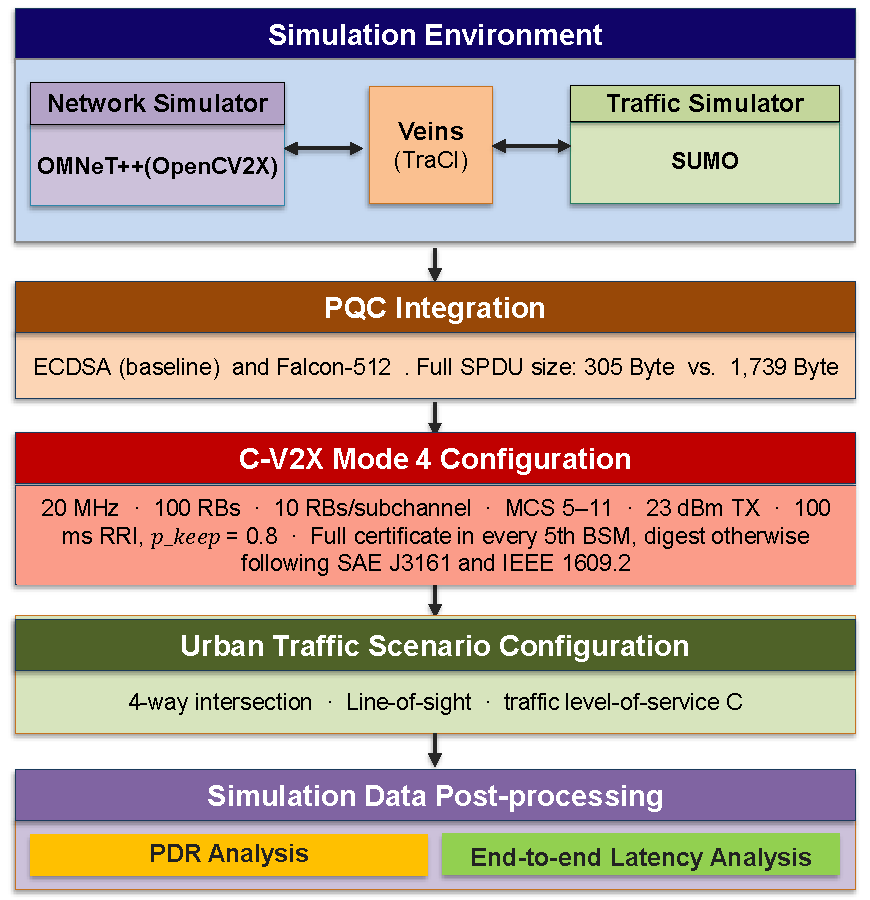
\includegraphics[width=\columnwidth]{figures/methodology_flowchart.pdf}
\caption{Comparative evaluation strategy between ECDSA P-256 and Falcon-512 for C-V2X PC5 Mode 4 sidelink communication.}
\label{fig:method}
\end{figure}

Sensing-based semi-persistent scheduling (SPS) enables vehicles in C-V2X PC5 Mode 4 to autonomously determine transmission resources. Each vehicle monitors the spectrum over a 1,000 ms sensing window. After that, each vehicle excludes resources exceeding a Received Signal Strength Indicator (RSSI) threshold and randomly selects from the remaining candidate resources. The selected resources are then reserved for a 100 ms Resource Reservation Interval (RRI) aligned with the BSM generation rate ~\cite{molina2017lte}. The SAE J3161-based configuration uses a 20 MHz sidelink channel with 100 resource blocks (RBs) in each 1 ms sidelink subframe. 10 RBs are grouped into a subchannel. The allowed Physical Sidelink Shared Channel (PSSCH) MCS indices range from 5 to 11, which determines the available transport block sizes (TBS) for carrying IEEE 1609.2 SPDUs \cite{sae_j3161}. This decentralized scheduling process improves communication scalability under nominal traffic conditions by reducing signaling overhead and avoiding frequent scheduling negotiations. However, the approach is highly sensitive to channel occupancy and transport block utilization because persistent reservations may repeatedly occupy overlapping resources across neighboring vehicles. The sensing-based SPS mechanism is particularly important in dense traffic because sidelink communication performance is strongly influenced by the interaction between packet size, reservation persistence, and resource reuse. When neighboring vehicles repeatedly reserve overlapping resources, the effective interference environment becomes increasingly correlated over time. As a result, communication degradation persists even when vehicles are physically close enough to maintain strong received signal power. This phenomenon differs from traditional wireless link degradation, dominated primarily by propagation loss or fading, and instead reflects the limitations of distributed resource coordination under constrained spectrum availability. These effects may become more severe in practical deployments where additional vehicular applications, such as cooperative perception, sensor data sharing, and automated driving coordination, share the same sidelink channel, increasing communication load beyond the baseline BSM exchange considered in this study. Since PQC artifacts enlarge every protected message, future high-bandwidth vehicular applications may experience compounded scalability challenges if spectrum-efficient authentication strategies are not incorporated into system design.

The TBS defines the maximum payload that can be carried in a single sidelink transmission. Under MCS 11 with a maximum allocation of 10 subchannels, the TB size is 2,481 bytes. The total size of an IEEE 1609.2 SPDU secured with Falcon-512 and carrying a full certificate is 1,739 bytes, comprising 57 bytes of protocol overhead, a 34-byte BSM payload, a 666-byte Falcon-512 signature, a 897-byte public key, and approximately 85 bytes of certificate-related overhead. By comparison, the size of an ECDSA SPDU with a full certificate is 305 bytes, a 5.7 times smaller payload. When only the certificate digest is transmitted, Falcon-512 reduces to 745 bytes versus 143 bytes for ECDSA, a 5.2 times reduction. Figure~\ref{fig:spdu_size} illustrates the SPDU sizes for both algorithms under full-certificate and digest-only transmission modes. This size difference directly determines subchannel consumption. At MCS 11, an ECDSA transmission with a full certificate requires 2 subchannels, while Falcon-512 requires 8 subchannels. Falcon-512 requires 4 subchannels while the certificate digest is transmitted, while ECDSA requires only 1~\cite{3gpp_36321}. This fourfold increase limits concurrent transmissions, raises channel utilization, and increases the probability that neighboring vehicles select partially overlapping resource reservations within the same sensing interval. Since Mode 4 scheduling decisions are made locally using sensing information without any instantaneous global channel knowledge, collisions created by increased spectrum occupancy may persist over several transmission cycles before reselection occurs, amplifying both instantaneous channel congestion and persistent collision probability in dense vehicular environments. Digest-based transmission reduces the per-message spectrum footprint but does not eliminate the penalty, since Falcon-512's signature alone remains substantially larger than a complete ECDSA SPDU.

\begin{figure}[t]
\centering
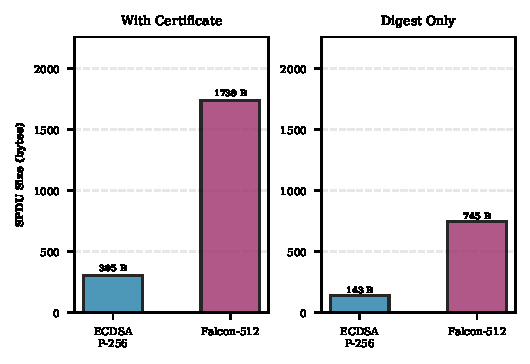
\includegraphics[width=\columnwidth]{figures/fig_spdu_size.pdf}
\caption{SPDU size comparison for ECDSA P-256 and Falcon-512 under full certificate and digest-only transmission modes.}
\label{fig:spdu_size}
\end{figure}

We evaluate a four-way urban intersection under line-of-sight (LoS) propagation conditions. Vehicle density is configured at 30 vehicles per kilometer, representing moderate urban arterial traffic with 2,172~vehicles per hour per approach, corresponding to level-of-service C as defined by the Highway Capacity Manual~\cite{HCM2016}. Vehicle's average speed is set to 45 mph. This scenario is selected as a representative moderate urban operating condition to serve as a foundational baseline for this evaluation. Table~\ref{tab:traffic_params} summarizes the urban traffic scenario used in this evaluation.

\begin{table}[ht]
\centering
\caption{Urban Traffic Scenario Configuration Utilized in this study}
\label{tab:traffic_params}
\renewcommand{\arraystretch}{1.2}
\begin{tabular}{ll}
\hline
\textbf{Parameter} & \textbf{Value} \\
\hline
Intersection type & Four-way urban intersection \\
Vehicle density & 30 vehicles/km \\
Traffic flow per approach & 2{,}172 vehicles/hour/approach \\
Traffic Level of Service & C \cite{HCM2016} \\
Average vehicle speed & 45 mph \\
\hline
\end{tabular}
\end{table}

Two performance metrics are evaluated. PDR is computed using the 5GAA P-190033 sliding-window method \cite{5gaa_p190033}: for each received packet at time $t$, a 5-second centered window $[t-2.5,\;t+2.5]$ s is applied to each transmitter-receiver pair. PDR is defined in Equation \eqref{eq:pdr}:

\begin{equation}
\label{eq:pdr}
\mathrm{PDR} =
\frac{N_{\mathrm{received}}}
{N_{\mathrm{transmitted}}}
\times 100\%
\end{equation}

where $N_{\mathrm{received}}$ is the number of successfully received packets within the evaluation window and $N_{\mathrm{transmitted}}$ is the total number of transmitted packets.

A mean PDR of 90\% or above is the accepted threshold for safety-critical vehicular applications \cite{twardokus2025chasm}. End-to-end latency measures the time from BSM creation at the sender application layer to reception at the receiver application layer, covering cryptographic processing, MAC-layer queuing, and radio propagation delays. This latency is measured for successfully received packets only. In this study, vehicles broadcast BSMs that are received by the RSU, and the reported latency represents the vehicle-to-RSU (i.e., vehicle-to-infrastructure [V2I]) communication delay. SAE J2945/1 specifies a maximum end-to-end latency of 100 ms for safety applications \cite{sae_j29451}.

\section{Results and Discussion}

This section presents the performance evaluation results and their corresponding interpretation, organized into the following four subsections. Section~\ref{sec:pdr} examines PDR as a function of transmitter-receiver distance and identifies the mechanisms driving this degradation. Section~\ref{sec:latency} presents the latency distributions and confirms that cryptographic processing contributes negligibly to end-to-end delay. Section~\ref{sec:spectrum} traces the PDR penalty to Falcon-512's increased subchannel consumption and sidelink resource contention. Section~\ref{sec:security} discusses deployment implications and mitigation strategies.

\subsection{Packet Delivery Ratio Performance}
\label{sec:pdr}
Figure \ref{fig:pdr_dist} presents PDR as a function of transmitter-receiver separation distance. ECDSA maintains near-perfect delivery at short ranges and exhibits a gradual, steady decline with increasing distance. It remains above the 90\% safety threshold \cite{twardokus2025chasm} out to 400 to 450 m range before dropping more sharply in the 450 to 700 m range, where path loss and interference from distant vehicles combine to reduce communication channel reliability.

\begin{figure}[!htbp]
\centering
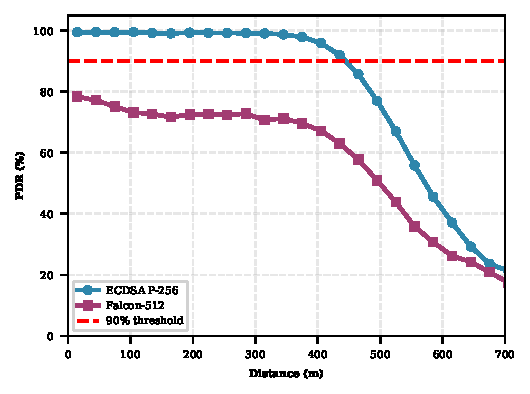
\includegraphics[width=\columnwidth]{figures/fig3_pdr_vs_distance.pdf}
\caption{PDR vs.\ distance for ECDSA P-256 and Falcon-512 under traffic level-of-service C with line-of-sight propagation. The dashed line at 90\% denotes the safety-critical PDR threshold.}
\label{fig:pdr_dist}
\end{figure}

Falcon-512, by contrast, shows noticeably reduced PDR, which is less than 90\% threshold, even within 0 - 100 m distance, a range in which ECDSA remains at or near 100\% PDR. This early degradation at short distances is particularly significant because it indicates that the PDR penalty for Falcon-512 is not primarily driven by propagation loss, which would affect both algorithms similarly, but by channel contention arising from its large packet size. As distance increases beyond 400 m, Falcon-512 declines steeply and consistently falls well below ECDSA, reaching very low PDR in the 400 to 700 m range.

However, the separation between the two curves does not widen continuously with distance; instead, the performance gap is most pronounced over short-to-mid ranges and narrows at longer ranges as ECDSA also experiences substantial link degradation. The fourfold subchannel overhead established in section~\ref{sec: method}, therefore, raises collision probability even between closely spaced vehicles, and these effects intensify as distance and propagation loss further reduce link margin. A 71\% mean PDR for Falcon-512 falls well below the 90\% safety-critical threshold, indicating that direct migration from ECDSA to Falcon-512 is not viable at 30 veh/km without mitigation strategies, such as a hybrid classical-PQC digital scheme and certificate segmentation.

The PDR results also show that successful post-quantum migration cannot be evaluated only through cryptographic execution time or signature verification success. In safety-critical vehicular communication, a cryptographic scheme is useful only if authenticated messages can be delivered with sufficient reliability and timeliness. Falcon-512 satisfies the authentication requirement for received packets, but its larger payload lowers the probability that packets are successfully delivered through the shared wireless channel. This distinction is important because a cryptographically strong scheme may still degrade system safety if its communication overhead prevents safety messages from reaching nearby road users.

\subsection{Latency Performance}
\label{sec:latency}
Figure \ref{fig:latency} and Table \ref{tab:results} present the end-to-end latency results. The latency distributions for ECDSA and Falcon-512 are nearly identical. The mean latency is around 52 ms for both ECDSA and Falcon-512. The 95th percentile latencies are around 96 ms for ECDSA and around 97 ms for Falcon-512. Both algorithms remain below the 100 ms maximum stipulated by SAE J2945/1 \cite{sae_j29451}. The boxplot confirms that the interquartile ranges, medians, and whisker extents are virtually indistinguishable between the two algorithms. This result confirms that Falcon-512's cryptographic computations add negligible overhead at the application layer under the evaluated conditions. Latency in both cases is dominated by MAC-layer queuing and radio transmission delays governed by the radio parameters rather than by the signature scheme. The near-identical latency distributions therefore indicate that Falcon-512 does not introduce a timing bottleneck for packets that are successfully delivered. Instead, the dominant performance loss occurs before successful reception, through increased collision probability and reduced channel reliability.

\begin{figure}[!htbp]
\centering
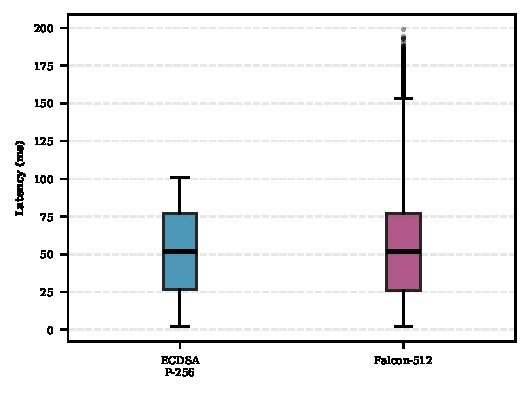
\includegraphics[width=\columnwidth]{figures/fig4_latency.pdf}
\caption{End-to-end latency distribution for ECDSA P-256 and Falcon-512 under traffic level-of-service C with line-of-sight propagation. Boxes represent the interquartile range (IQR), with the central horizontal line denoting the median, and whiskers are drawn at 1.5 × IQR beyond the box edges.}
\label{fig:latency}
\end{figure}

Taken together, the PDR and latency results establish an important distinction between timeliness and reliability. Falcon-512 can meet the latency requirements for delivered packets, but it does not meet the reliability requirements under the evaluated roadway traffic density. This outcome is critical for safety-critical V2X applications, where timely arrival is necessary but insufficient. Safety messages must also be delivered with high probability to nearby receivers. Therefore, the main deployment barrier is not whether Falcon-512 can be verified quickly enough but whether Falcon-512-authenticated messages can be transmitted frequently and reliably enough in a congested sidelink environment.

\begin{table}[t]
\centering
\caption{Performance Comparison under traffic level-of-service C with line-of-sight propagation}
\label{tab:results}
\begin{tabular}{lcc}
\toprule
\textbf{Metric} & \textbf{ECDSA} & \textbf{Falcon-512} \\
\midrule
Packet Size, Cert (B)         & 305   & 1,739 \\
Packet Size, Digest (B)       & 143   & 745   \\
Mean Latency (ms)             & 52 & 52 \\
95th Percentile Latency (ms)  & 96    & 97    \\
Mean PDR$^{\dagger}$ (\%)    & 95 & 71 \\
Verification Success (\%)     & 100   & 100   \\
\bottomrule
\multicolumn{3}{l}{\footnotesize $^{\dagger}$5GAA~P-190033 sliding-window method~\cite{5gaa_p190033}}
\end{tabular}
\end{table}

\subsection{Spectrum Resource Utilization Analysis}
\label{sec:spectrum}
As the SPDU size breakdown in Figure~\ref{fig:spdu_size} illustrates, the impact of Falcon-512 on C-V2X Mode 4 performance is fundamentally driven by increased spectrum resource consumption rather than computational overhead. The increased resource demand directly reduces the number of simultaneous transmissions that can coexist within the shared sidelink channel. Falcon-512's larger transport block allocation reduces the number of candidate resources available for neighboring vehicles and increases the probability that multiple vehicles will reserve overlapping resources. Since SPS reservations persist for multiple transmission intervals, these collisions may continue across consecutive scheduling periods, further amplifying channel congestion effects.

Figure~\ref{fig:pdr_dist} shows that degradation appears for Falcon-512 even at short transmitter-receiver distances where propagation loss remains relatively small. This behavior indicates that the primary cause of Falcon-512's performance degradation is spectrum contention rather than wireless channel attenuation. Since Falcon-512 increases the physical layer resource allocation required for each transmission, fewer orthogonal scheduling opportunities remain available within each sidelink subframe. This reduction in effective multiplexing capacity increases resource overlap among transmitting vehicles and raises the likelihood of packet collisions even when the received signal strength remains sufficiently strong for successful decoding under isolated transmission conditions. When the communication distance increases, propagation loss combines with increased collision probability and resource scarcity. These results demonstrate that spectrum efficiency becomes a dominant constraint for post-quantum cryptographic deployment in decentralized vehicular sidelink communication systems.

These observations additionally suggest that post-quantum communication scalability may become increasingly challenging as vehicular density rises. Under higher traffic densities, the sidelink resource pool becomes progressively saturated even under conventional ECDSA-based operation. Because Falcon-512 consumes multiple subchannels per transmission, the effective channel capacity available for concurrent users decreases substantially. As a result, the communication system reaches congestion conditions at significantly lower vehicle densities compared to classical cryptographic operations. This scalability limitation is particularly important for future intelligent transportation deployments involving cooperative perception, platooning, and high-frequency sensor-sharing applications, where communication reliability requirements are more strict and channel utilization is already expected to increase. In such environments, spectrum-efficient post-quantum authentication mechanisms may become essential for maintaining both security and communication reliability simultaneously.

\subsection{Security and Deployment Implications}
\label{sec:security}
The PDR and end-to-end latency analysis of this study have important implications for the deployment of PQC in future vehicular communication systems. Although Figure~\ref{fig:latency} establishes that Falcon-512 satisfies the computational latency requirements of safety-critical V2X applications, its substantially larger packet size introduces significantly high spectrum efficiency penalties under decentralized sidelink scheduling, which contributed to its 71\% overall PDR. These findings indicate that direct replacement of ECDSA with PQC signatures may not be feasible in dense traffic environments without additional cross-layer modifications or congestion mitigation mechanisms.

One potential migration strategy involves hybrid certificate architectures combining classical and post-quantum cryptographic mechanisms~\cite{mamun_pqc}. Short-term pseudonym certificates may continue using compact classical signatures to preserve spectrum efficiency, while long-term trust anchors and certificate provisioning infrastructures employ PQC to provide protection against future quantum-capable adversaries~\cite{twardokus2024cryptography}. Infrastructure-assisted certificate dissemination through RSUs may also reduce repeated sidelink transmission of large public key certificates and improve channel efficiency.

Digest-based certificate transmission can reduce repeated certificate overhead, but it does not fully solve the resource problem because Falcon-512 signatures remain substantially larger than ECDSA signatures even when the full public key certificate is not included. Therefore, practical deployment may require a combination of techniques, including certificate caching, RSU-assisted certificate distribution, adaptive certificate transmission intervals, and congestion-aware message scheduling. Such approaches would reduce redundant certificate transmission and preserve more sidelink resources for safety-critical messages.

The results additionally highlight important considerations for future vehicular communication standards. Existing standards such as IEEE 1609.2 and SAE J3161 were originally designed around compact ECDSA and do not explicitly account for the significantly larger payloads introduced by PQC schemes. Future revisions may therefore require adaptive congestion control, dynamic resource allocation, optimized certificate distribution strategies, and cross-layer communication-aware security mechanisms to support scalable quantum-resistant vehicular communication deployments.

The presented findings also demonstrate that future quantum-resistant vehicular communication standards cannot rely solely on cryptographic substitution at the application layer. Instead, communication-aware security co-design may become necessary, where cryptographic selection, certificate transmission frequency, congestion control, and sidelink scheduling are jointly optimized. Such cross-layer considerations are likely to become increasingly important as vehicular communication systems evolve toward higher-bandwidth cooperative driving and autonomous transportation applications.

\section{Conclusion and Future Work}


This paper presents a performance evaluation strategy and conducts a quantitative assessment of Falcon-512 post-quantum signatures on C-V2X Mode 4 sidelink under moderate roadway traffic density. Results show that while Falcon-512 remains computationally feasible under the evaluated conditions, the 5.7 times packet size overhead causes about 23\% mean PDR degradation from 95\% to 71\%, dropping Falcon-512 well below the 90\% safety-critical threshold. Falcon-512 fits within SAE J3161 TBS limits without protocol modifications, satisfying a critical backward-compatibility requirement. Both algorithms remain well within the 100 ms SAE J2945/1 latency limit, confirming that the deployment barrier is spectral rather than computational. This study also demonstrates that direct ECDSA-to-Falcon migration at this density requires mitigation strategies, such as digest-based certificates, hybrid cryptographic schemes, or infrastructure-assisted distribution. More broadly, the presented results illustrate that post-quantum migration in vehicular communication systems is not solely a cryptographic transition problem but also a communication scalability problem. The interaction between cryptographic payload size, decentralized sidelink scheduling, and shared spectrum utilization fundamentally influences whether quantum-resistant authentication can be deployed without degrading safety-critical communication reliability. The presented findings further suggest that future quantum-resistant vehicular communication systems will require joint optimization across cryptography, wireless communication, congestion control, and resource scheduling layers rather than isolated security upgrades at the application layer alone.

The present study focused on Falcon-512 under a single moderate-density, line-of-sight urban intersection scenario. Future evaluations should therefore consider additional post-quantum schemes, multiple traffic densities, non-line-of-sight propagation, and fully distributed vehicle-to-vehicle reception patterns. Future work will extend our current evaluation across low-density suburban traffic, moderate urban traffic, and highly congested urban scenarios to characterize how post-quantum communication overhead scales with channel load and vehicle population. Additional studies will incorporate urban canyon environments, multipath fading, shadowing, and heterogeneous mobility conditions to evaluate the robustness of post-quantum communication performance under more realistic deployment conditions. Future investigations should also evaluate additional post-quantum signature schemes, including Dilithium-2, SPHINCS+, and hybrid ECDSA+Falcon architectures, to establish comparative communication performance tradeoffs across multiple cryptographic candidates. Further work may additionally explore adaptive certificate dissemination, infrastructure-assisted distribution through roadside units and cellular connectivity, dynamic congestion-control strategies, and cross-layer communication-aware security optimization methods. Together, these efforts aim to develop scalable deployment guidelines for quantum-resistant vehicular communication systems and support the evolution of future IEEE and SAE standards toward practical post-quantum V2X security architectures.

% \section*{Acknowledgment}
% This material is based upon the work supported by the National Center for Transportation Cybersecurity and Resiliency (TraCR) headquartered at Clemson University, Clemson, South Carolina, USA. Any opinions, findings, conclusions, and recommendations expressed in this material are those of the author(s) and do not necessarily reflect the views of TraCR, and the U.S. Government assumes no liability for the contents or use thereof. 

\bibliographystyle{IEEEtran}
\bibliography{references}

\end{document}
